\section{Setup and preliminaries} \label{sec:pre}
\subsection{Definitions and model}
Throughout the paper we look at curved folded surfaces as piecewise $C^2$ developable surfaces, whose discontinuities are focused along creases. We assume that these creases are $C^2$ curves that may intersect one another, and we call these intesection points \textit{vertices}. These curves segment the surface into various disconnected components, which we call curved patches. By our assumptions these curved patches remain $C^2$, i.e. though the folding operation creates discontinuities along patches, the patches viewed separately are deformed by $C^2$ deformations. We model each patch as a discrete orthogonal geodesic net, and the entire surface by keeping appropriate boundary constraints between the patches and along the creases as done in \cite{rabi2018shape} but also support vertices, a trivial extension that is discussed at \secref{sec:app}. Throughout the paper we will often visualize the crease pattern itself, i.e. the initial flatten surface together with its curved creases (\figref{fig:crease_pattern}). If $S$ is a curved folded surface with a given crease pattern, we call a crease \textit{active} at $S$ if there is a discontinuity along it (TODO:point to a figure).

\begin{figure} [h]
	\centering
	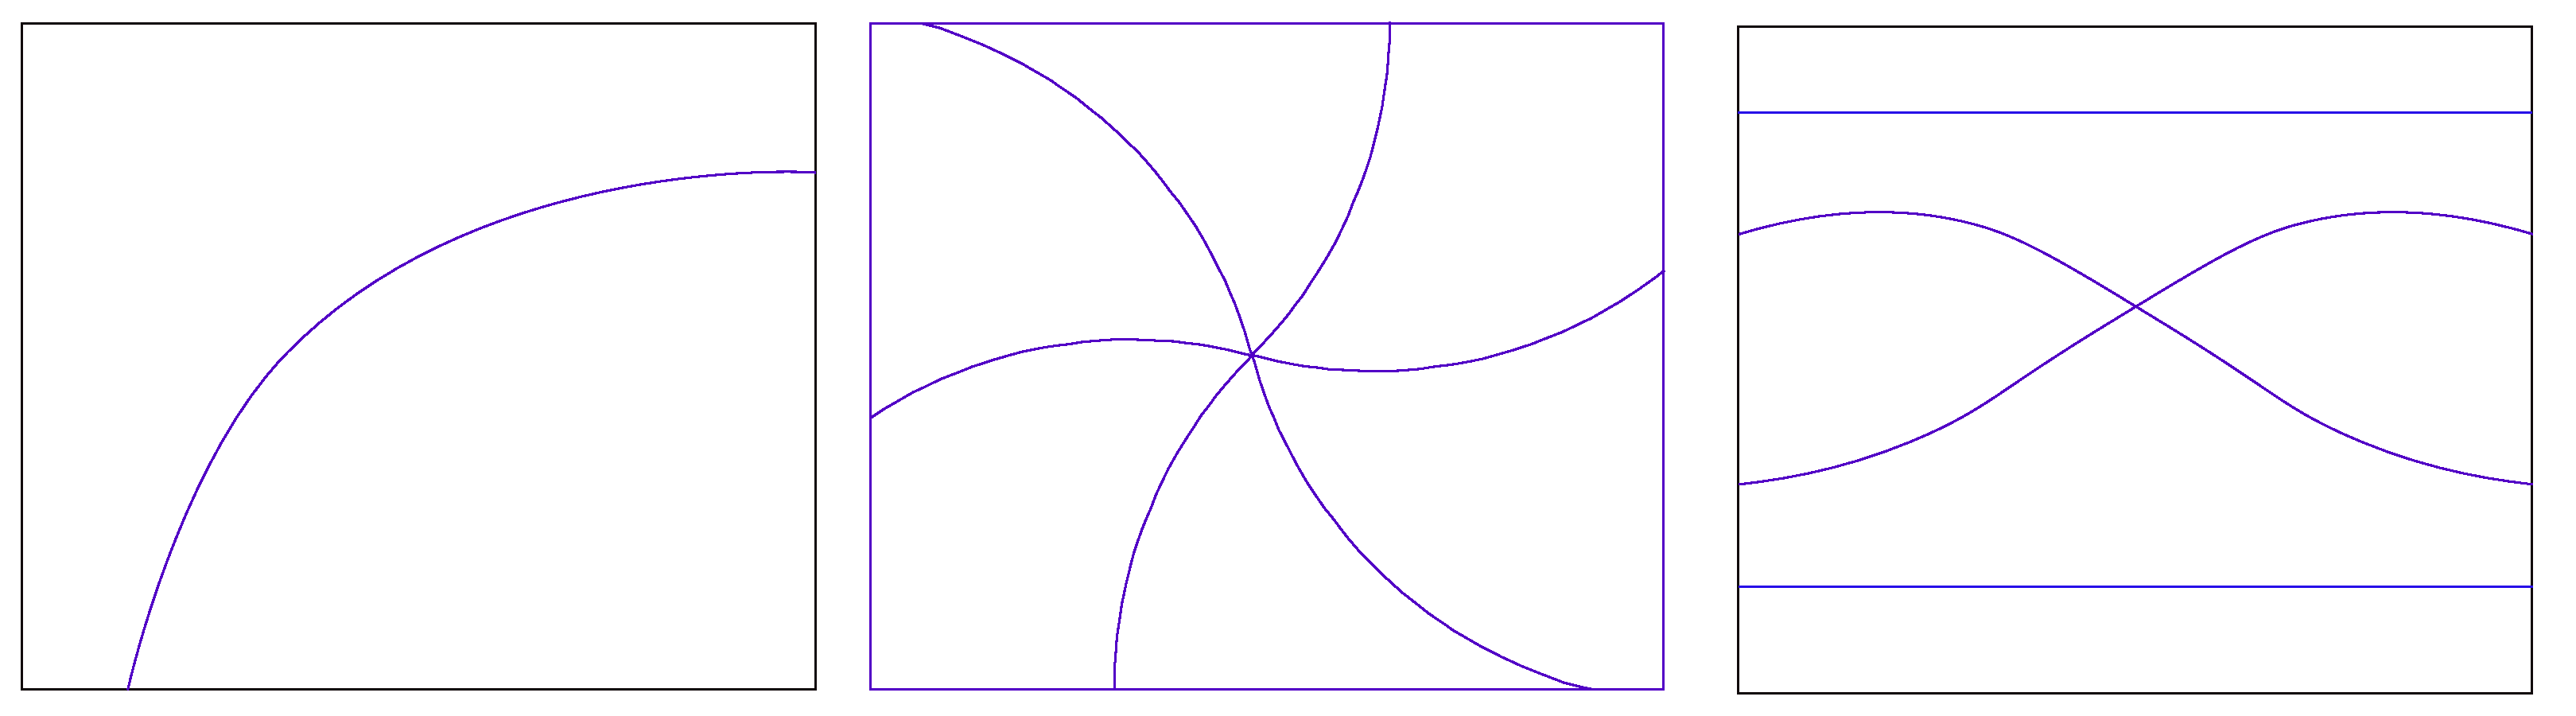
\includegraphics[width=\linewidth]{figures/crease_patterns}
	\caption{Curved and straight crease patterns, decomposing a pattern into multiple components and intersecting at vertices.}
	\label{fig:crease_pattern}
\end{figure}

\subsection{Curved folding from the view of the crease} \label{sec:curved_folding_from_a_curve}
Let $\Gamma(t)$ be a curve on a smooth developable surface $S$,  let $\gamma(t)$ be its flattened curve, $k(t)$ its curvature, and $k_g(t)$ its geodesic curvature such that $k_g(t) = k(t) \cos(\alpha(t))$ for some $\alpha \neq 0$. This implies that at each point along $\Gamma(t)$, the tangent planes of $S$ make an angle of $\alpha$ with the osculating planes of $\Gamma(t)$. One can switch this point of view: start with a flat curve $\gamma(t)$, isometrically embed the curve in $\mathbb{R}^3$ and construct a developable surface by reconstructing the planes at each point. As long as the crease is curved, i.e. has some normal curvature such that $k(t) > k_g(t)$ and $\alpha(t) \neq 0$ then there are 2 distinct planes containing $\Gamma'(t)$ and forming an angle of $\alpha(t)$ with the curve's osculating plane. Therefore, one can locally construct two different smooth developable surfaces passing through $\Gamma(t)$ with $\gamma(t)$ as its flattening. Alternatively, one can construct a folded surface by a consistent smooth choice of a different tangent plane for each "side" of the curve (see Fig. \ref{fig:curved_fold_through_curve}) \cite{more_on_paper}. The tangent planes from both sides are reflections of one another through the osculating plane of the curve \cite{curved_folding_kilian}.

\begin{figure} [h]
	\centering
	\includegraphics[width=0.7\linewidth]{figures/curved_fold_through_curve.pdf}
	\caption{(TODO BETTER FIG) Left: A flattened curve in 2D. Right: A small neighbourhood around an embedding of the curve in $\mathbb{R}^3$, its osculating plane and two options to extend a the curve to developable surface by constructing the 2 planes containing the curve's tangent and making an angle of $\alpha(t)$  with the osculating plane. Choosing 2 different tangents along each 'side' of the curve creates discontinuities along the curve and a curved folded surface.}
	\label{fig:curved_fold_through_curve}
\end{figure}